%%% LaTeX Template: Two column article
%%%
%%% Source: http://www.howtotex.com/
%%% Feel free to distribute this template, but please keep to referal to http://www.howtotex.com/ here.
%%% Date: February 2011

%%% Preamble
\documentclass[	DIV=calc,%
							paper=a4,%
							fontsize=11pt,%
							twocolumn]{scrartcl}	 					% KOMA-article class

\usepackage{lipsum}													% Package to create dummy text

\usepackage[english]{babel}										% English language/hyphenation
\usepackage[protrusion=true,expansion=true]{microtype}				% Better typography
\usepackage{amsmath,amsfonts,amsthm}					% Math packages
\usepackage[pdftex]{graphicx}									% Enable pdflatex
\usepackage[svgnames]{xcolor}									% Enabling colors by their 'svgnames'
\usepackage[hang, small,labelfont=bf,up,textfont=it,up]{caption}	% Custom captions under/above floats
\usepackage{epstopdf}												% Converts .eps to .pdf
\usepackage{subfig}													% Subfigures
\usepackage{booktabs}												% Nicer tables
\usepackage{fix-cm}													% Custom fontsizes



%%% Custom sectioning (sectsty package)
\usepackage{sectsty}													% Custom sectioning (see below)
\allsectionsfont{%															% Change font of al section commands
	\usefont{OT1}{phv}{b}{n}%										% bch-b-n: CharterBT-Bold font
	}

\sectionfont{%																% Change font of \section command
	\usefont{OT1}{phv}{b}{n}%										% bch-b-n: CharterBT-Bold font
	}



%%% Headers and footers
\usepackage{fancyhdr}												% Needed to define custom headers/footers
	\pagestyle{fancy}														% Enabling the custom headers/footers
\usepackage{lastpage}	

% Header (empty)
\lhead{}
\chead{}
\rhead{}
% Footer (you may change this to your own needs)
\lfoot{\footnotesize \texttt{http://proactive.activeeon.com/} \textbullet ~Big Data Landscape}
\cfoot{}
\rfoot{\footnotesize page \thepage\ of \pageref{LastPage}}	% "Page 1 of 2"
\renewcommand{\headrulewidth}{0.0pt}
\renewcommand{\footrulewidth}{0.4pt}



%%% Creating an initial of the very first character of the content
\usepackage{lettrine}
\newcommand{\initial}[1]{%
     \lettrine[lines=3,lhang=0.3,nindent=0em]{
     				\color{DarkBlue}
     				{\textsf{#1}}}{}}



%%% Title, author and date metadata
\usepackage{titling}															% For custom titles

\newcommand{\HorRule}{\color{DarkBlue}%			% Creating a horizontal rule
									  	\rule{\linewidth}{1pt}%
										}

\pretitle{\vspace{-30pt} \begin{flushleft} \HorRule 
				\fontsize{50}{50} \usefont{OT1}{phv}{b}{n} \color{DarkOrange} \selectfont 
				}
\title{Big Data Landscape}					% Title of your article goes here
\posttitle{\par\end{flushleft}\vskip 0.5em}

\preauthor{\begin{flushleft}
					\large \lineskip 0.5em \usefont{OT1}{phv}{b}{sl} \color{DarkOrange}}
\author{Ge Song, Nicolas Narbais, }											% Author name goes here
\postauthor{\footnotesize \usefont{OT1}{phv}{m}{sl} \color{DarkBlue} 
					ActiveEon 								% Institution of author
					\par\end{flushleft}\HorRule}

\date{}																				% No date



%%% Begin document
\begin{document}
\maketitle
\thispagestyle{fancy} 			% Enabling the custom headers/footers for the first page 
% The first character should be within \initial{}
\initial{E}\textbf{xecutive Summary: }


\section*{\color{DarkOrange}Introduction}

\subsection*{Challenges of Big Data processing}\label{sec: challenges}

\subsection*{Real-time processing for data streams}
 

\section*{\color{DarkOrange}Parallel Data Processing}

\initial{P}arallel computing is a computation model which uses two or more processors (cores or computers) in combination to perform multiple operations concurrently. The basic condition for parallel computing is that in general, a large problem can be divided into a limited number of smaller problems, and these smaller problems can be handled simultaneously.
					
Unlike the traditional serial computation, parallel computing uses multiple resources simultaneously to solve a problem. The problem should first be cut into a series of instructions, which will later be executed simultaneously on different processors. This model is much more suitable for explaining, modeling and solving complex real world phenomena. It does not only speed up the time spent to perform a large task, but also makes it possible to process large-scale data sets or complex problems which cannot be handled by a single machine.
					
In parallel computing, there are mainly two forms of parallelism: 
\begin{itemize}
\item Data Parallelism

\item Task Parallelism

\end{itemize}
					
We will introduce them separately in the coming section. 

\subsection*{Two types of parallelisms}

\textbf{Data parallelism} focuses on distributing data across different parallel computing resources, in which the same computation is applied to multiple pieces of data. This is usually used for data-intensive tasks. Fig. \ref{fig:data_para} shows the schematic of data parallelism.

\begin{figure}
  \centering
    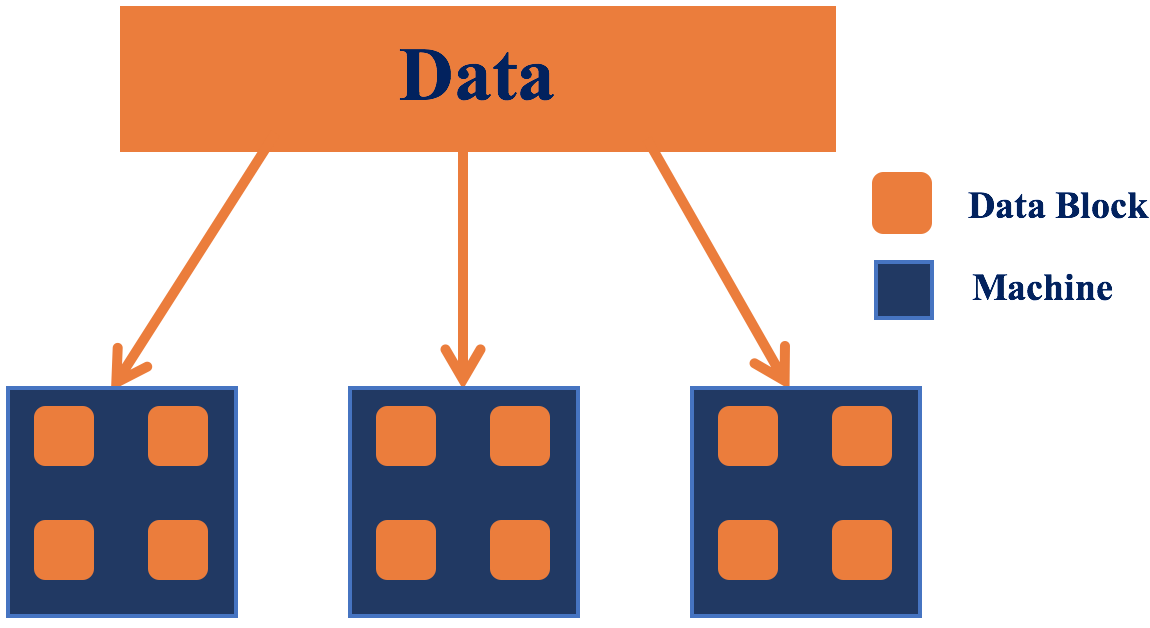
\includegraphics[width=0.4\textwidth]{images/data_para.png}
    \caption{Data Parallelism Schematic}
    \label{fig:data_para}   
\end{figure}

In a data parallelism process, the data set is first divided into partitions, which will later be processed by different processors using the same task. This simple idea makes the storing and handling of big data possible. For example, Facebook has several million photos uploaded each day. But these photos are too large to be stored in a single machine. Then a data parallelism strategy is suitable for this problem.

However, because each machine only has a subset of data, gathering the results together is a problem that this model needs to address. At the same time, the main factor affecting the performance of this model is the transmission of intermediate data, hence reducing the amount of data to be transferred is another problem to face.
Since data parallelism emphasizes the parallel and distributed nature of data, when the size of data is growing, it is inevitable to use this model in parallel computing. Examples of Big Data frameworks that uses data parallelism are: Hadoop MapReduce \cite{1}, Apache Spark\cite{2}, YARN\cite{3}, and Apache Storm\cite{4}.

\textbf{Task parallelism} focuses on distributing tasks concretely performed by processors across different parallel computing resources, in which the same data (or maybe different data in a hybrid system) is processed by different tasks. This is usually used for computation-intensive tasks.

In a task parallelism process, the parallelism is organized around the functions to be run rather than around the data. It depends on task decomposition. This idea makes it possible to handle a complex problem. 
%For example, in a semantic join, task 1 needs to save the data which meets a certain condition in a specific data structure, and task 2 needs to use the data which meets another condition to probe this data structure. This process can be considered as a task parallel process.

The difficulties of this type of process lie first on the decomposition of the work, specifically the decomposition of queries in a join process. Also task parallelism processes usually suffer from bad load balancing, since it is not easy to divide tasks with equal complexity. The communication among tasks is another problem. Synchronization is the most important communication approach in task parallelism processes, and can be divided into thread synchronization and data synchronization. Thread synchronization focuses on determining the order of execution in order to avoid Data Race Condition problems. Data synchronization is mainly used to ensure the consistency among multiple copies of data.

Recently, the most popular task parallelism example is deep learning. Deep learning is a branch of machine learning which is based on a set of algorithms which attempt to model high-level abstractions in data by using multiple processing layers. The difference between deep learning and traditional machine learning is that in deep learning instead of having one model to train all the data, we separate the model into layers, and each layer can be considered as a sub-task of the whole model.

The most common combination of data parallelism and task parallelism is pipelining. Suppose you have multiple tasks, task I, task II and task III, instead of having each one operating on the data independently, pipelining takes the data and first give it to task I, then task II and finally task III. Image processing often chooses to use a pipeline. Images are coming in a stream, some of the processing starts with the first task, and applies a certain filter on the images, then passes on to the second task, and so on. 
%This is a very common combination of task parallelism and data parallelism. 
An example of pipeline processing of images is shown in Fig. \ref{fig:task_para}.

\begin{figure}
  \centering
    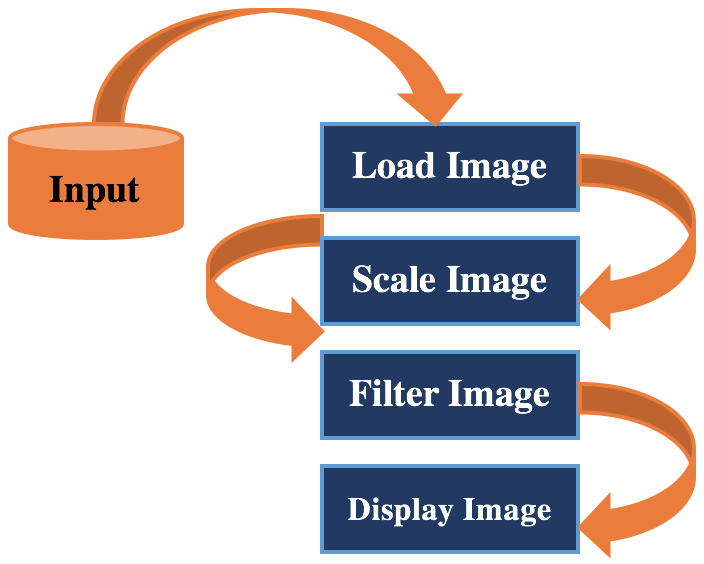
\includegraphics[width=0.4\textwidth]{images/task_para.png}
    \caption{Images Pipeline Processing}
    \label{fig:task_para}   
\end{figure}

Task parallelism and data parallelism complement each other, and they are often used together to tackle large-scale data processing problems. The Big Data frameworks that use task parallelism are: Apache YARN \cite{3} and Apache Storm \cite{4}. They are hybrid systems which support both task and data parallelism.


\subsection*{Big Data processing systems}

\textbf{MapReduce} is a flexible and scalable parallel and distributed programming paradigm which is specially designed for data-intensive processing. It was initially introduced  by Google \cite{Dean:2004:MSD:1251254.1251264} and popularized by the Hadoop framework. 

The concept of MapReduce has been widely known since 1995 with the message passing Interface (MPI) \cite{MPI} standard, having \emph{reduce}  and \emph{scatter} operations. %\footnote{\url{http://mpitutorial.com/tutorials/mpi-reduce-and-allreduce/}} 
 %\footnote{\url{http://mpitutorial.com/tutorials/performing-parallel-rank-with-mpi/}}.
 The MapReduce programming model is composed of a Map procedure and a Reduce procedure. The Map task is usually used for performing some preliminary and cleaning work such as filtering and sorting. For example we can use a Map task to sort the students by alphabetical order of their surname, and then filter the students whose score is below a certain level. The Reduce task is used to perform a summary operation such as count or aggregation. For example we can use a Reduce task to count the number of students whose score is above a given level.  

The idea of the MapReduce paradigm comes from high-order functional programming, where Map and Reduce are two primitives. In this paradigm every record is represented by a $<key, value>$ pair. The Map function processes a fragment of $<key, value>$ pairs in order to generate a list of intermediate $<key, value>$ pairs. Each $<key, value>$ pair is processed by the same map function on different machines without depending on other pairs. The output keys of the Map tasks could be either the same as the input keys or different from them. The output $<key, value>$ pairs have an information of partition which indicates to which Reduce task this pair needs to be sent. The partition information makes sure that all pairs with the same key can be later sent to the same Reduce task. The Reduce function gathers the outputs of the same partition from all map tasks together through a Shuffle phase and merges all the values associated with the same key, then produces a list of $<key, value>$ pairs as output. 

\begin{figure}
  \centering
    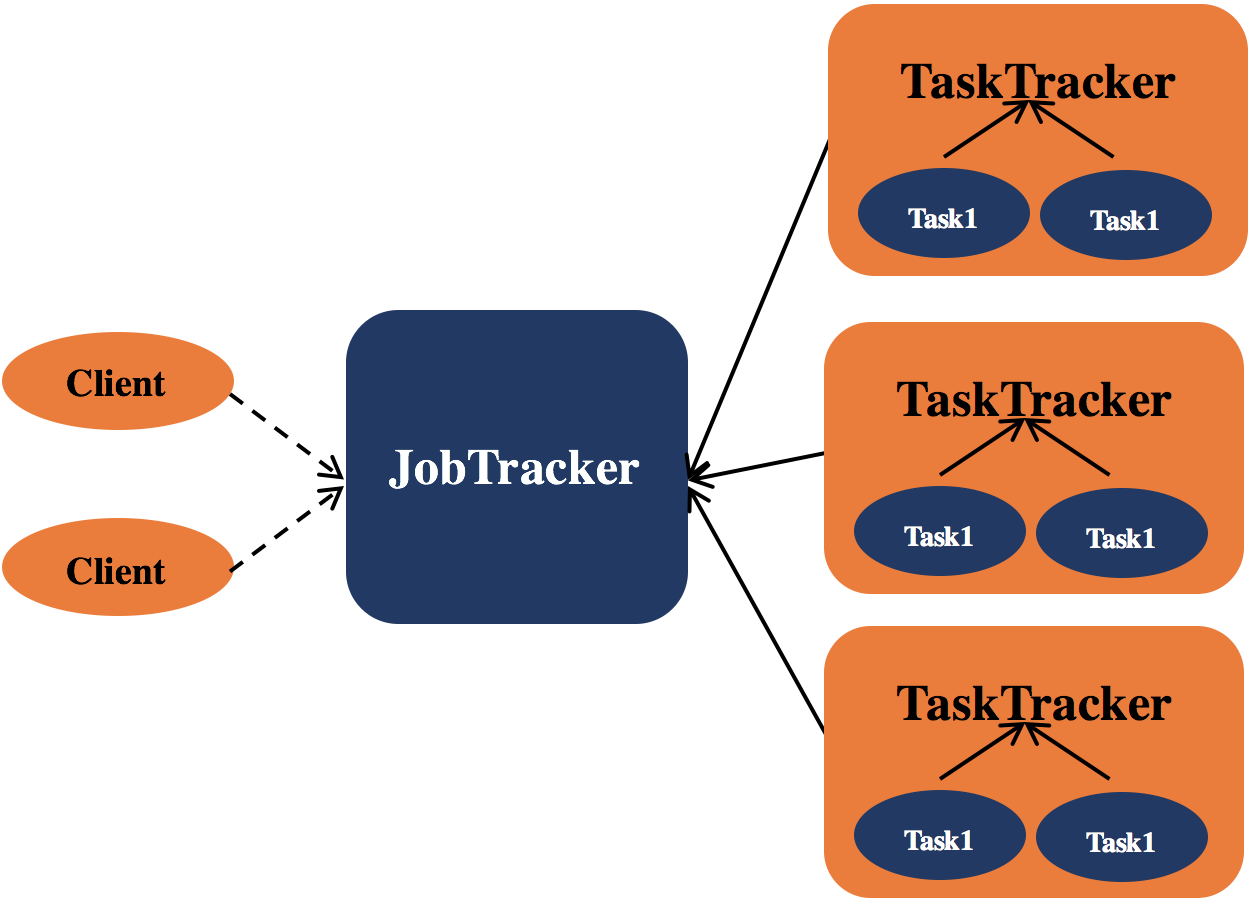
\includegraphics[width=0.4\textwidth]{images/mapreduce.png}
    \caption{Physical Structure of Hadoop System}
    \label{fig:MapReduce0}   
\end{figure}

\textbf{Hadoop} \cite{2} is an open-source framework written in Java for distributed storing and processing large scale data sets. The core of Hadoop contains a distributed storage named Hadoop Distributed File System (HDFS), and the MapReduce programming paradigm. HDFS is a distributed, scalable, and portable file-system written in Java. It stores large files across multiple machines on a cluster. Its reliability is achieved by replicating the data among multiple nodes. The default number of replications is set to 3, which means the same piece of data is stored on three nodes. 
It is very popular not only among the academic institution but also in many companies such as web search, social network, economic computation and so on. A lot of research work focuses on optimizing Hadoop performance and its efficiency in many different aspects.

The whole system of Hadoop works in a master-slave manner, with JobTracker as the master, and the other nodes as slaves. A TaskTracker daemon runs on each slave node. 
The JobTracker daemon is responsible for resource allocation (e.g. managing the worker nodes), tracking (e.g. resource consumption or resource availability) and management (e.g. scheduling). 
The TaskTracker has much more simple responsibilities. It is in charge of launching tasks with an order decided by the JobTracker, and sending the task status information back to JobTracker periodically. The schematic of this process is shown in Fig.~\ref{fig:MapReduce0}.



When running a Hadoop job, input data will first be divided into some splits (64M by default). Then each split will be processed by a user-defined map task. 

So the whole process of a Hadoop job as shown in Fig.~\ref{fig:MapReduce1} can be summarized as follow:

\begin{itemize}

\item \textbf{Step 1:} Split data into blocks (64M by default)

\item \textbf{Step 2:} Map Phase: Extract information from data (filter, sort)

\item \textbf{Step 3:} Shuffle Phase: Exchange data through network from Map Phase to Reduce Phase

\item \textbf{Step 4:} Reduce Phase: Summary operation (count, aggregation)

\end{itemize}


\begin{figure*}
  \centering
    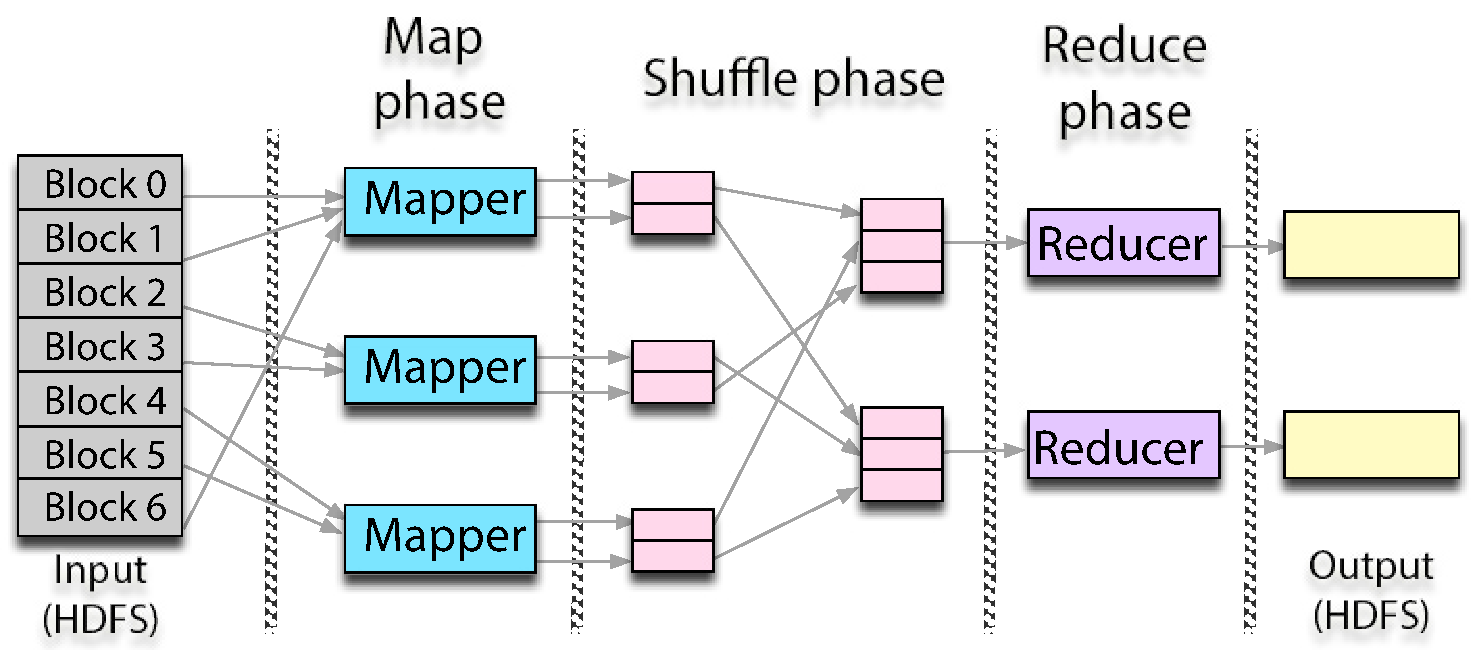
\includegraphics[width=0.8\textwidth]{images/map_reduce.pdf}
    \caption{Logical View of Hadoop Framework}
    \label{fig:MapReduce1}   
\end{figure*}


The previous introduction on Hadoop shows that a Hadoop MapReduce job has some special characteristics as shown below,

\begin{itemize}
\item \textbf{Execution Similarity:} According to the programming model, users only have to provide a map function and a reduce function. And the execution for each Map task (or Reduce task) is very similar to others. In other words, all data will be processed by these functions repeatedly. Thanks to this design, we only need to study how each $<key, value>$ pairs are processed for a particular job, as reading, sorting, transferring and writing data are independent of these two functions.

\item \textbf{Data Similarity:} MapReduce is well suited for off-line batches processing. And it is usually used to do repeated work in which the input data has very similar format, such as log analysis, inverted index and so on. We can just take a look at a small sample and then we can estimate the whole dataset.
\end{itemize}

Hadoop is now a very mature system, with specific application and user groups. However, due to the limitation of the MapReduce paradigm and the Hadoop implementation, it has performance limitations in some application scenarios. In order to better integrate Hadoop in the applications, 
many works have been done from the very beginning to extend Hadoop and to improve its performance. We discuss a limited number of them.

The whole system of Hadoop works in a master-slave manner, with JobTracker as the master, and the other nodes as slaves. A TaskTracker daemon runs on each slave node. The JobTracker daemon is responsible for resource allocation (e.g. managing the worker nodes), tracking (e.g. resource consumption or resource availability) and management (e.g. scheduling). The TaskTracker has much more simple responsibilities. It is in charge of launching tasks with an order decided by the JobTracker, and sending the task status information back to JobTracker periodically. The schematic of this process is shown in Fig. 2.3.
When running a Hadoop job, input data will first be divided into some splits (64M by default). Then each split will be processed by a user-defined map task.
So the whole process of a Hadoop job as shown in Fig. 2.4 can be summarized as follow:

\begin{itemize}

\item \textbf{Step 1:} Split data into blocks (64M by default)

\item \textbf{Step 2:} Map Phase: Extract information from data (filter, sort)

\item \textbf{Step 3:} Shuffle Phase: Exchange data through network from Map Phase to Reduce Phase

\item \textbf{Step 3:} Reduce Phase: Summary operation (count, aggregation)

\end{itemize}

The previous introduction on Hadoop shows that a Hadoop MapReduce job has some
special characteristics as shown below,

\begin{itemize}

\item \textbf{Execution Similarity:} According to the programming model, users only have to provide a map function and a reduce function. And the execution for each Map task (or Reduce task) is very similar to others. In other words, all data will be processed by these functions repeatedly. Thanks to this design, we only need to study how each < key,value > pairs are processed for a particular job, as reading, sorting, transferring and writing data are independent of these two functions.

\item \textbf{Data Similarity:} MapReduce is well suited for off-line batches processing. And it is usually used to do repeated work in which the input data has very similar format, such as log analysis, inverted index and so on. We can just take a look at a small sample and then we can estimate the whole dataset.


\end{itemize}


Hadoop is now a very mature system, with specific application and user groups. However, due to the limitation of the MapReduce paradigm and the Hadoop implementation, it has performance limitations in some application scenarios. In order to better integrate Hadoop in the applications, many works have been done from the very beginning to extend Hadoop and to improve its performance, mainly through the following three ways:

\begin{itemize}

\item Improve the performance of Hadoop by predicting its performance and tuning the parameters.

\item Extend Hadoop to have database-like operations.

\item Combine with other programming language or model.

\end{itemize}

\textbf{Apache Spark} \cite{2} is another popular parallel computing framework after Hadoop MapReduce. Spark provides an application programming interface in Java, Scala, Python and R on a data structure called the resilient distributed dataset (RDD). Spark also uses the MapReduce paradigm but it overcomes the limitations in MapReduce. Hadoop MapReduce forces a particular linear data flow, it reads input data from disk, maps a function across the data, reduces the results of the map, and stores reduction results on disk. The resilient distributed dataset structure works as a working set for distributed programs, it offers a restricted form of distributed shared memory. Unlike Hadoop jobs, the intermediate data of Spark can be saved in memory, which avoids the unnecessary reading and writing from HDFS. Therefore Spark is better for data mining and machine learning algorithms, which require iterations. RDD facilitates the implementation of iterative algorithms which need to visit the dataset multiple times in a loop. It also makes it easy to do interactive or exploratory data analysis, like repeated database-style querying of data.
Spark requires a manager which is in charge of the cluster, and a distributed file system. Spark also supports a pseudo distributed mode (local mode), which is usually needed for testing.

Compared with Hadoop, Spark has the following advantages:

\begin{figure}
  \centering
    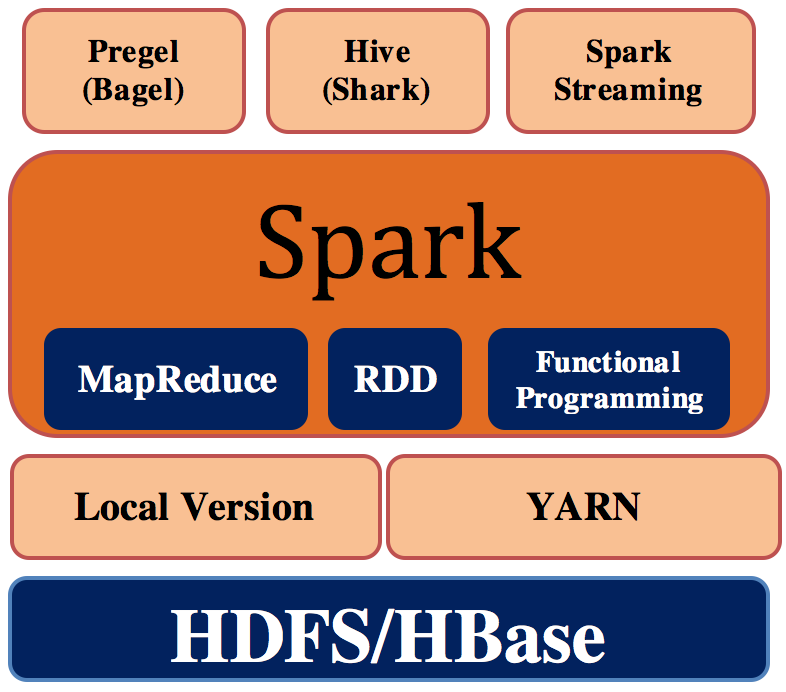
\includegraphics[width=0.5\textwidth]{images/spark.png}
    \caption{Structure of Spark System.}
    \label{fig:Spark}   
\end{figure}

\begin{itemize}

\item Store intermediate data into memory, providing a higher efficiency for iterative opera- tions. So Spark is more suitable for Data Mining and Machine Learning algorithms containing a lot of iterations.

\item Spark is more flexible than Hadoop. It provides many operators like: map, filter, flatMap, sample, groupByKey, reduceByKey, union, join, cogroup, mapValues, sort, partionBy, while Hadoop only provides Map and Reduce. However, due to the char- acteristics of RDD, Spark does not perform well on the fine-grained asynchronous update applications or the applications with incremental changes, such as the web crawlers with updates.

\item By providing a wealth of Scala, Java, Python APIs and interactive Shell API, Spark has a higher availability with different programming languages and different modes to use.

\end{itemize}

According to the characteristics of Spark, its applicable scenarios are:

\begin{itemize}
\item Iterative calculations requiring multiple operations

\item Applications that require multiple operations on a specific data set

\end{itemize}

And the benefit increases with the amount of data and the number of operations. But the benefit is smaller in applications with a small amount of data and intensive computations.
The structure of a Spark system is shown in Fig. \ref{fig:Spark}.

\textbf{YARN} \cite{3} is an attempt to take Apache Hadoop beyond MapReduce for data-processing. As we explained above, in Hadoop, the two major responsibilities of the JobTracker are resource management and job scheduling or monitoring. As there is only one JobTracker in the whole system, it becomes a bottleneck. The fundamental idea of YARN is to split these functions into two separate daemons --- a global ResourceManager (RM) and a per-application ApplicationMaster (AM).

\begin{figure}
  \centering
    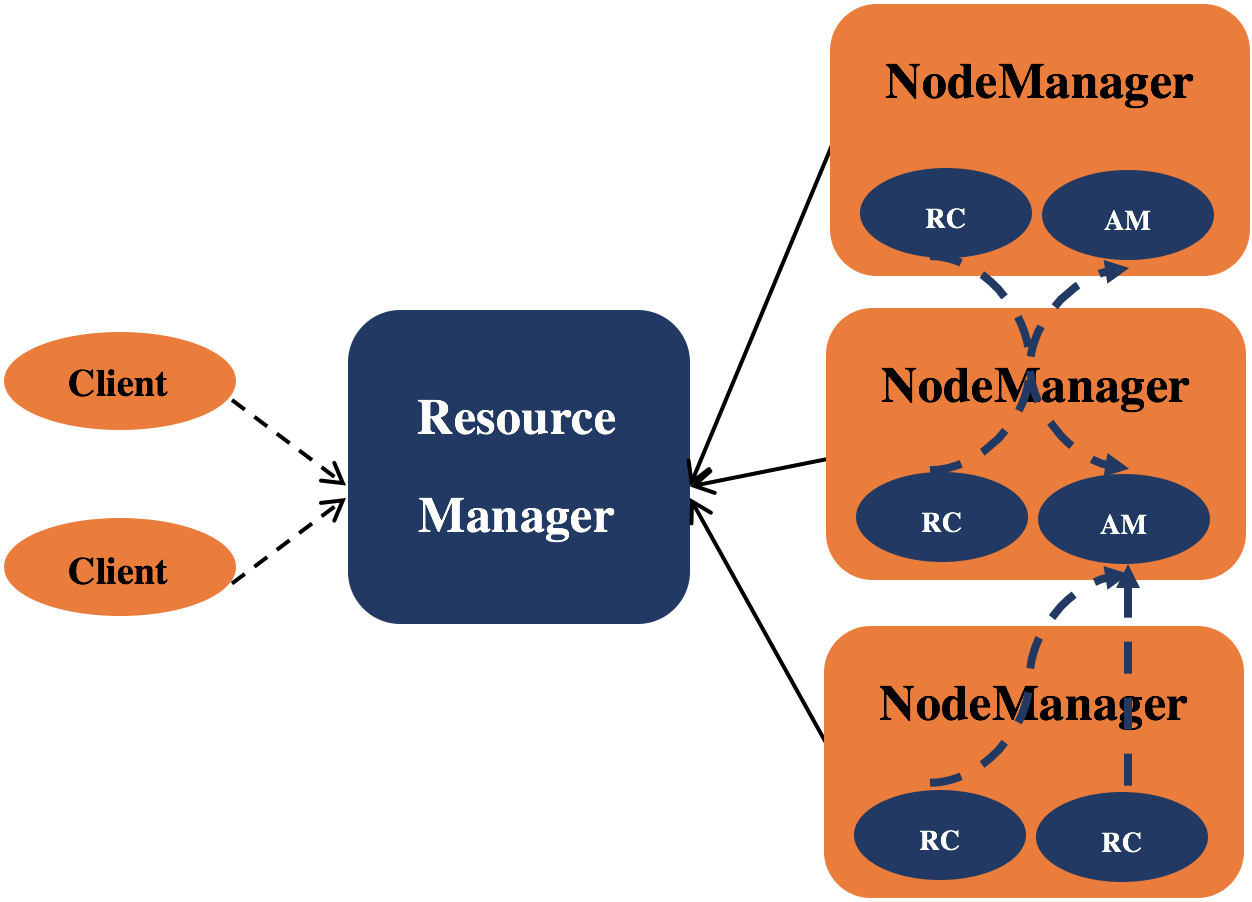
\includegraphics[width=0.4\textwidth]{images/YARN.png}
    \caption{Architectural View of YARN}
    \label{fig:YARN}   
\end{figure}

The ResourceManager together with the per-node slave daemon NodeManger forms a new generic system for managing tasks in a distributed manner. Moreover, the ResourceManager is the ultimate authority that arbitrates resources among all applications in the system, while the per-application ApplicationMaster is a framework specific entity and is used to negotiate resources from the master ResourceManager and the slaves NodeManagers to execute and monitor the tasks. A pluggable Scheduler is used in the ResourceManager to allocate resources to jobs. The Scheduler works using an abstract concept of Resource Container (RC) which incorporates resource elements such as CPU, Memory, Disk, Network etc. The NodeManager is a per-node slave daemon, and its responsibility is to launch the tasks and to monitor the resources (CPU, Memory, Disk, Network). From the system perspective, the ApplicationMaster runs as a normal container.
An architectural view of YARN is shown in Fig.~\ref{fig:YARN}.

\textbf{Hadoop}, \textbf{Spark} and \textbf{YARN} all use the \textbf{MapReduce} paradigm as their abstract computational concept. The ecosystem of MapReduce and its derivative methods are mature and very good for parallel processing of big data. But most of them are still an `offline' processing platform, which means that they can not handle dynamic data streams.



\subsection*{Parallel data warehouse}

\subsection*{ETL for Big Data}


\section*{\color{DarkOrange} Real-time Data Processing}

As we introduced in the Introduction Section, the characteristics of Big Data contains 4 Vs, among which Volume, Variety and Velocity are the most important. The relations among these 3 Vs are shown in Fig.~\ref{fig:3v}.

\begin{figure}
  \centering
    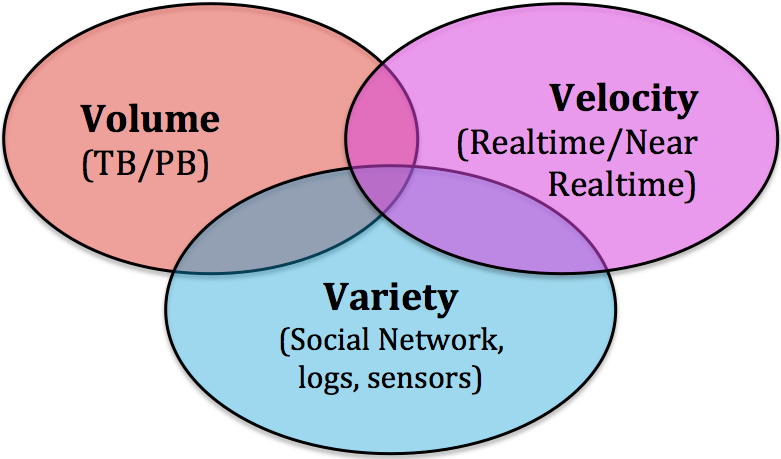
\includegraphics[width=0.4\textwidth]{images/3v.png}
    \caption{The 3 Vs of Big Data}
    \label{fig:3v}   
\end{figure}

The need of velocity requires to process the data fast, so that the system can react to the changing conditions in  real time. This requirement of processing high-volume data streams with low-latency becomes increasingly important in the areas of trading, fraud detection, network monitoring, and many other aspects, thus increasing the demand for stream processing. Under this requirement, the capacity of processing big volumes of data is not enough, we also need to react as fast as possible to the update of data.

Stream processing is a programming paradigm, which is also called dataflow programming or reactive programming. A stream is a sequence of data and a series of operations will be applied to each element in the stream. Data items in streams are volatile, they are discarded after some time. Since stream processing often involves large amount of data, and requires the results in real-time, the stream processing platforms (e.g. Apache Storm) often work in parallel. Besides, this paradigm is a good complement of parallel processing, and allows applications to more easily exploit a limited form of parallel processing.  

Traditional popular big data processing frameworks like Hadoop and Spark assume that they are processing data from a data storage that all data is available when it is needed. And it may require several passes over a static, archived data. But when data arrives in a stream or streams, data will be lost if it is not processed immediately. Moreover, in the streaming scenarios, usually the data arrives so rapidly that it is not feasible to store it all in a conventional database, to process be processed when needed. So stream processing algorithms often rely on concise, approximate synopses of the input streams which can be computed with a simple pass over the streaming data.

In the coming sections of this part, we will first introduce the rules for processing Data Streams, then we will present several Data Stream management systems, and a detailed introduction about Apache Storm can be found in the end.

%Below, we will first present the issues in data stream processing, then introduce an approach to summarize a stream with only looking at fixed-length windows, and in the end we will present some Stream management systems.

\subsubsection*{Rules in Data Stream processing}


A \textbf{data stream} is a real-time, continuous, ordered (explicitly by timestamp or implicitly by arrival time) sequence of items.


%The most notable characteristic of a data stream is that it often delivers elements very rapidly. So we must process the data in real time, or we lose the opportunity to process it forever. So it is very important to execute the algorithm in memory with no or rare accesses to secondary storage.

In general, we need to follow some rules for processing low-latency and high-volume data streams. The most important rules are:

\begin{itemize}

\item \textbf{Rule 1: Keep the data moving} \\
The first requirement for a real-time high-volume data stream processing framework is to process data ``on the fly", without storing everything. 

\item \textbf{Rule 2: Handle Stream Imperfections}\\
The second requirement is to provide resilience results against ``imperfections" in streams, including delay, missing and out-of-order of data.

\item \textbf{Rule 3: Generate Predictable Outcomes}\\
A stream processing engine must guarantee predictable and repeatable outcomes. 

\item \textbf{Rule 4: Integrate Stored and Streaming Data }\\
A stream processing system also needs to efficiently store, access, and modify state information, and combine it with new coming streaming data. 

\item \textbf{Rule 5: Guarantee Data Safety and Availability}\\
Fault-tolerance is another important point for such a system.

\item \textbf{Rule 6:  Partition and Scale Applications Automatically}\\
In order to meet the real-time requirement for high-volume and fast-changing data streams, the capability to distribute processings across multiple machines to achieve incremental scalability is also important. Ideally, the system should automatically and continuously distribute the data and queries.

\item \textbf{Rule 7: Process and Respond Instantaneously}\\
The last but most important requirement is to have a highly-optimized, minimal-overhead execution engine to deliver real-time response for high-volume applications.
\end{itemize}

When designing a stream processing algorithm, we need to keep two things in mind:

\begin{itemize}

\item It can be more efficient to get an approximate answer than an exact solution.

\item A variety of techniques related to hashing turn out to be very useful. Because, these techniques introduce useful randomness, which produces an approximate answer that is very close to the exact one.

\end{itemize}

The approximation of a streaming algorithm comes from two aspects: (1) from limiting the size of states maintained for the process; (2) from reducing the precision of the result. 

The algorithms for processing streams usually involve summarization of the stream in some ways. Summary data structures such as : wavelets, sketches, histograms and samples have been widely used especially  for streaming aggregation. These algorithms always begin by considering how to make a useful sample or how to filter out most of the undesirable elements. Another important approach to summarize a stream is to process within a fixed-length window, then query the window as if it were a relation in a database. This model is called ``Sliding Window Model" \cite{SlidingWindow}.

%The parallel and distributed streaming algorithm should also be both time and space efficient in order to manage high-speed data streams, and also communication efficient to deal with physical data distribution.

A lot of prior work on stream processing focused on developing space-efficient, one-pass algorithms for performing a wide range of centralized, one-shot computations over massive streams. These applications involve: (1) computing quantiles; (2) estimating distinct values; (3) counting frequent elements; (4) estimating join sizes and stream norms.

As the size of data is getting larger, some recent efforts have concentrated on distributed stream processing and proposing communication efficient streaming frameworks to handle a number of query tasks such as aggregation, quantiles and join (such as Apache Storm, Spark Streaming, Yahoo! S4 etc.) which will be introduced in the next Section.  


\subsection*{Data Stream management systems}

 \begin{table*}[]
\centering
\caption{A comparison of Storm, Spark Streaming and Yahoo! S4}
\label{tab:compare}
\begin{tabular}{@{}|c|c|c|c|@{}}
\toprule
                                                                                            & \textbf{Storm}    & \textbf{\begin{tabular}[c]{@{}c@{}}Spark\\ Streaming\end{tabular}} & \textbf{S4}      \\ \midrule
\textbf{Original Design}                                                                    & Twitter           & UC Berkeley                                                        & Yahoo!           \\ \midrule
\textbf{Implemented In}                                                                     & Clojure           & Scala                                                              & Java             \\ \midrule
\textbf{APIs}                                                                               & Java (and others) & Scala, Java                                                        & Java             \\ \midrule
\textbf{Processing Model}                                                                   & Record at a time  & Mini Batches                                                       & Record at a time \\ \midrule
\textbf{Latency}                                                                            & Sub-Second        & Few Seconds                                                        & Sub-Second       \\ \midrule
\textbf{Data Units}                                                                         & Tuple             & Java Object                                                        & Java Object      \\ \midrule
\textbf{Hadoop Distribution}                                                                & Hortonworks HDP   & Cloudera, MapR                                                     & None             \\ \midrule
\textbf{Resource Manager}                                                                   & Mesos/Zookeeper   & YARN/Mesos                                                         & Zookeeper        \\ \midrule
\textbf{Distributing Work}                                                                  & User Specifies    & MapReduce                                                          & Evenly           \\ \midrule
\textbf{\begin{tabular}[c]{@{}c@{}}Fault Tolerance\\ (Ever Record Processed:)\end{tabular}} & At Least Once     & Exactly Once                                                       & No Guarentee     \\ \midrule
\textbf{Dynamic Deployment}                                                                 & Yes               & No                                                                 & No               \\ \bottomrule
\end{tabular}
\end{table*}

There are many efforts towards build a Data Stream processing system. 
Some works have extended the MapReduce paradigm to process dynamic data. But these frameworks are not suitable for processing data streams and returning the results in real-time because of the nature of MapReduce paradigm.

To address the limitation, some stream processing engines have been proposed, some of them are centralized which are not able to process a huge volume of data streams. Others are parallel. 
Among all the parallel frameworks, \textbf{Spark Streaming}, \textbf{Yahoo! S4} and \textbf{Twitter Storm} are the most widely used. % parallel and distributed stream  processing framework. 
We will introduce them separately.

 
 \textbf{Spark Streaming} is an extension of the Spark framework. It enables scalable, high-throughput and fault-tolerant stream processing for dynamic data streams. Spark Streaming receives input data streams and divides them into batches, which will later be processed by the Spark engine to generate final stream in batches. It has APIs for Scala, Java and Python. Spark Streaming is a data parallelism framework. It follows the same ideas as MapReduce batch processing paradigm. It is not a real ``real-time processing" framework: the incoming events are cached and processed as a batch, resulting in a larger delay than the real streaming processing frameworks such as Twitter Storm.

\textbf{Yahoo! S4}  is a general-purpose, distributed, scalable, partially faut-tolerant, pluggable platform for data stream processing that allows users to easily develop applications for processing continuous unbounded streams of data. It is a java based solution which relies on the user defined classes to process and produce stream data. It uses Apache Zookeeper \cite{DBLP:conf/usenix/HuntKJR10} to maintain the state of a distributed job. It allows a parallel execution of data streams. But it does not provide a dynamic load balancing protocol, which is left for users to define. S4 uses "Plain Old Java Objects" (POJO) mode as its communication protocol and User Datagram Protocol (UDP) as its underlying protocol, which has an impact on reliability. Besides, it does not support dynamic deployment of the cluster or add or delete nodes during run time.

 \textbf{Twitter Storm} \cite{Toshniwal:2014:STO:2588555.2595641}, is a distributed, parallel and fault tolerance framework for data streams processing. Queries can be expressed in using the boxes and arrows model. A Storm job, which is called a Topology, consists in two components: Spout and Bolt . Spout nodes are responsible for generating the system input streams. Bolt nodes are in charge of processing those streams and generate output results. It relies on Zookeeper servers to maintain the state of distributed setups. Storm supports task parallelism. In a Storm cluster, the data is flowing while the tasks do not. Storm is a real "flow processing" framework: every incoming data will be handled as an event, which has a smaller delay than the mini-batch processing frameworks such as Spark Streaming. It also supports dynamic deployment of the cluster, and add or delete nodes during run time.
 
 Table.~\ref{tab:compare} shows a comparison of these three frameworks.

Through the above comparison, we think Storm is the best choice for a real-time and low latency data stream processing problem. The reasons are:

\begin{itemize}

\item Storm processes data in form of streams. And it processes intensive queries in parallel. (Latency)

\item It is scalable. As the amount of data increases, we can simply increase the number of nodes for processing. (Dynamic Deployment) 

\item It has a good reliability, which can ensure that each event can be at least processed once. (Fault Tolerance)

\item It provides good fault tolerance. Once a node fails, the task on this node is re-assigned to the other nodes. (Fault Tolerance)

\item It provides a simple programming model, which reduces the complexity of real-time processing. (Distributing Work)

\item It supports multiple programming languages such as Clojure, Java, Ruby and Python. (APIs)

\end{itemize}

We will give a detailed introduction about Apache Storm in the coming section.


\subsection*{Introduction to Apache Storm}

Storm is a distributed, reliable, fault-tolerant framework for data streams processing. It was firstly developed in Twitter, and is now an Apache open source project.

A Storm job is called a \textbf{Topology}. A Topology is made of different types of components. Each component is responsible for a simple specific task. The component for handling and distributing the input streams is called a \textbf{Spout}. The component for processing the streams is called a \textbf{Bolt}. A Spout passes data to Bolt(s), which transforms it in some ways. A Bolt is a user defined task, it can either persist the data into different sort of storages, or pass it to some other Bolts, or process it through some user specified functions. A Storm cluster can be seen as a chain of a Spout followed by several Bolts, where each Bolt makes some kind of transformation on the data. An example of a Topology is shown in Fig.~\ref{fig:topology}.

\begin{figure}
  \centering
    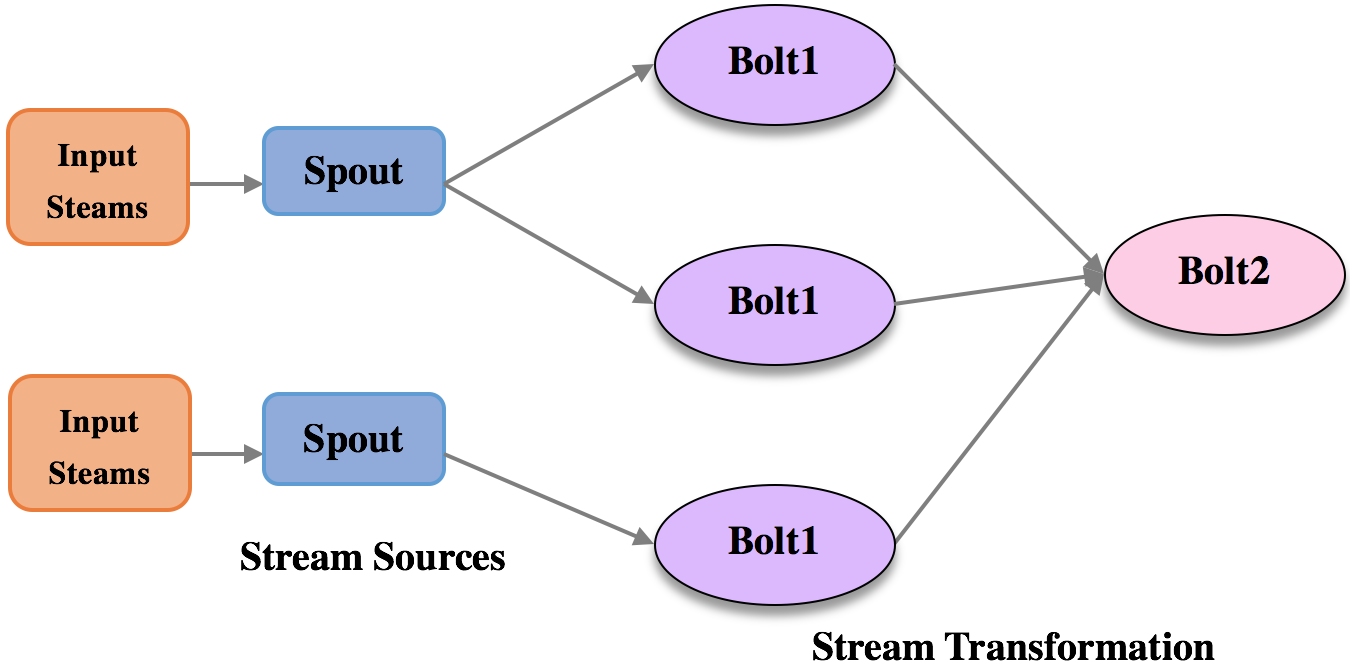
\includegraphics[width=0.8\textwidth]{topology.png}
    \caption{An example of a Topology}
    \label{fig:topology}   
\end{figure}

A Storm cluster works in a master slave manner. A daemon called Nimbus runs on the Master node. It is responsible for distributing the user specified code to the cluster: assigning tasks to worker nodes, and monitoring the cluster for failures. A daemon called Supervisor runs on the Worker nodes. It executes the task on this node and is part of the Topology. Usually, a Topology runs across many worker nodes. Storm keeps the states of the cluster in Zookeeper or on local disk. So the daemons are stateless. They can fail or restart without affecting the health of the whole system. The physical view of a Storm cluster is shown in Fig.~\ref{fig:stormcluster}

\begin{figure}
  \centering
    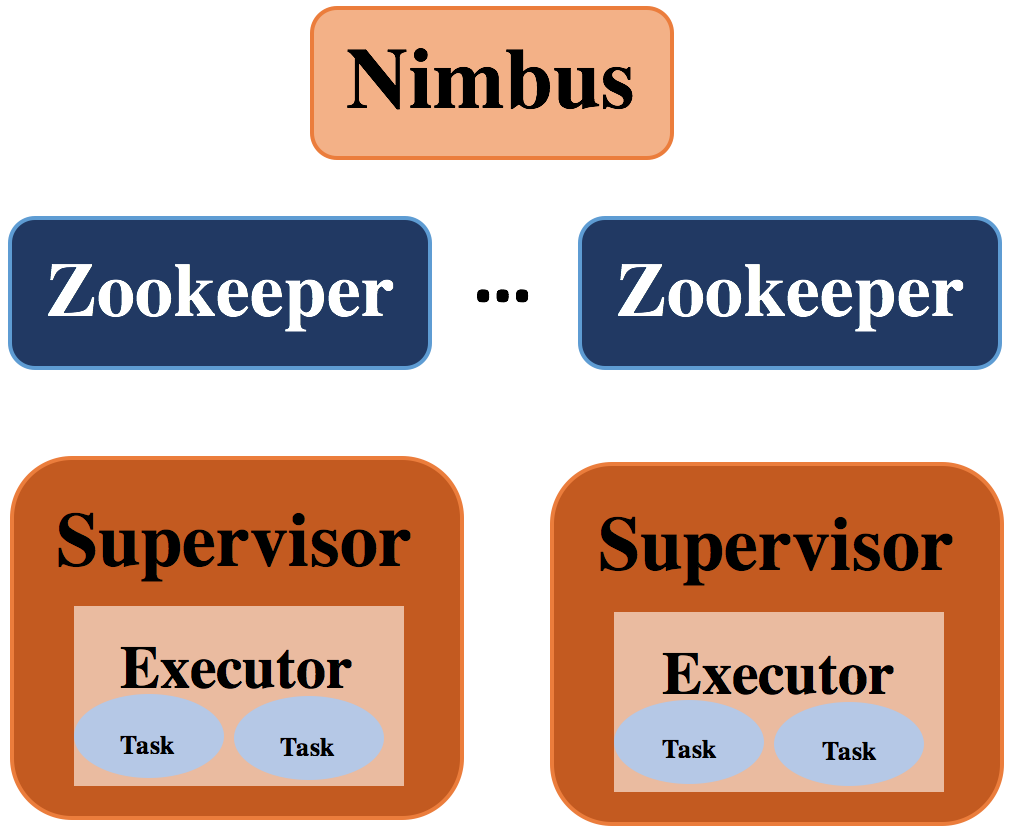
\includegraphics[width=0.5\textwidth]{stormcluster.png}
    \caption{A physical view of a Storm cluster}
    \label{fig:stormcluster}   
\end{figure}

\section*{\color{DarkOrange} ProActive}

\subsection*{Introduction to ProActive}

\subsection*{Role of ProActive in Big Data area}

\subsection*{Advantages of using ProActive}

\bibliographystyle{unsrt}
\bibliography{biblio}

\end{document}

